\documentclass[10pt,a4paper]{article}
%\usepackage{minted}

\usepackage{amsmath}
\usepackage{amsthm}

\usepackage{amsfonts}
\usepackage{amssymb}
\usepackage{graphicx}
\usepackage{float}
\usepackage{hyperref}
\usepackage{cleveref}
\usepackage{todonotes}
\newcommand{\ii}[0]{\mathrm{i}}
\newcommand{\RR}[0]{\mathbb{R}}
\newcommand{\bx}[0]{\mathbf{x}}
\newcommand{\bw}[0]{\mathbf{w}}
\newcommand{\bu}[0]{\mathbf{u}}
\newcommand{\bC}[0]{\mathbf{C}}
\newcommand{\bF}[0]{\mathbf{F}}
\newcommand{\bI}[0]{\mathbf{I}}
\newcommand{\bA}[0]{\mathbf{A}}
\newcommand{\bbf}[0]{\mathbf{f}}
\newcommand{\lib}[1]{\subsection*{\textcolor{blue}{#1}}}

\theoremstyle{definition}
\newtheorem{definition}{Definition}[section]
 
 
\usepackage{pgfplots}


\newcommand{\by}[0]{\mathbf{y}}

\newcommand{\sinc}[0]{\mathrm{sinc}}
\usepackage{amsthm}
\newtheorem{lemma}{Lemma}
\newtheorem{theorem}{Theorem}

\newtheorem{remark}{Remark}

\title{A Unified Numerical Approach to Nonlocal Operators Induced by L\'evy Process \\  \large Applications to the Fractional Laplacian, Nonlocal Diffusion and Jump Diffusion for Option Pricing}
\date{}
%\author{Kailai Xu}
\begin{document}

\lib{$\mathcal{H}$ Matrix}

For completeness, we discuss the hierarchical matrix technique. Especially we give a detailed description on the storage format, construction, fast matrix vector multiplication routine and LU decomposition. We later show how to construct the $\mathcal{H}$ matrix from kernels. 

The discretization of the jump diffusion part $\int_\RR (u(x+y)-u(y))dy$ will usually lead to a dense matrix, which typically requires $\mathcal{O}(N^2)$ storage and has $\mathcal{O}(N^2)$ complexity for matrix-vector multiplication, $\mathcal{O}(N^3)$ for LU decomposition. Many techniques, such as the panel clustering methods and the fast multipole methods were developed. Later $\mathcal{H}$-matrix was considered by W.~Hackbusch and many variations of hierarchical matrices have been intensively studied by researchers. $\mathcal{H}$-matrices can reduces the storage and arithmetics to nearly optimal complexity $\mathcal{O}(N)$ up to $\log N$ scaling. It relies on the fact that the kernel functions are smooth in the off diagonal. 

\subsection{Construction and Storage}

The construction of the $\mathcal{H}$ matrices can be best described in terms of matrix indices and the geometric points. Each entry $A_{ij}$ represents the interaction between two nodes $x_i$ and $x_j$. Let $I$, $J\subset \mathbb{N}$ be row and column index sets, then $A_{IJ}=(a_{ij})_{i\in I, j\in J}$ describes the interaction between a cluster $X_I = \{x_i\}_{i\in I}$ and another cluster $X_J = \{x_j\}_{j\in I}$. The interaction kernel function $k(x,y)$ is assumed to be smooth for sufficiently large $|x-y|$. 

Typically, it requires $\mathcal{O}(|I||J|)$ complexity to store the interaction data. However, if we assume that $I\subset J=\emptyset$ and geometrically the clusters $X_I$, $X_J$ are separate in the sense of admissibility

\begin{definition}
	For two sets of indices $I$ and $J$ and the associated cluster $X_I$, $X_J$; assume that the kernel is asymptotically smooth, the admissibility condition is given by
	\begin{equation}\label{equ:adm}
		\min\{\mathrm{diam}(X_I),\mathrm{diam}(X_J) \}\leq \eta \mathrm{dist}(X_I,X_J)
	\end{equation}
	where $\mathrm{diam}(X_I) = \max_{x_i,x_j\in X}|x_i-x_j|$ AND $\mathrm{dist}(x_i,x_j)=\min_{x_i\in X_I, x_j\in X_J}|x_i-x_j|$. If the condition \cref{equ:adm} is not satisfied, we say $X_I$ and $X_J$ or $I$ and $J$ are inadmissible. 
\end{definition}

In our numerical examples, we use $\eta=1$, which indicates adjacent clusters are inadmissible since the distance is always zero. 

The admissible blocks usually have low rank structures. This is best illustrated by an example. Suppose $k(x,y)=\frac{1}{|x-y|^2}$, and further assume $x\in X_I$, $y\in X_J$. Assume $X_I$ and $Y_J$ are inadmissible, and $\bar x\in \mathcal{X}$, where $\mathcal{X}$ is the convex hull of $X_I$. Then we have
\[\frac{1}{{|x - y{|^2}}} = \frac{1}{{|x - \bar x - (y - \bar x){|^2}}} = \frac{1}{{|y - \bar x{|^2}{{\left| {\frac{{x - \bar x}}{{y - \bar x}} - 1} \right|}^2}}}\]

Since 
\[\left| {\frac{{x - \bar x}}{{y - \bar x}}} \right| < 1\]
we have 
\[\frac{1}{{|y - \bar x{|^2}{{\left| {\frac{{x - \bar x}}{{y - \bar x}} - 1} \right|}^2}}} = \frac{1}{{|y - \bar x{|^2}}}\left( {1 + \frac{{x - \bar x}}{{y - \bar x}} + {{\left( {\frac{{x - \bar x}}{{y - \bar x}}} \right)}^2} +  \ldots } \right)\]
which is in the form of 
\begin{equation}
	\frac{1}{{|x - y{|^2}}} = \sum_{n=0}^\infty \alpha_n(x-\bar x)\beta_n(y-\bar x)
\end{equation}

Then series is convergent and therefore the residual term will decay. It is possible to approximate $\frac{1}{{|x - y{|^2}}}$ with a few terms
\begin{equation}
	\frac{1}{{|x - y{|^2}}} \approx \sum_{n=0}^r \alpha_n(x-\bar x)\beta_n(y-\bar x)
\end{equation}
And therefore the interaction matrix for the cluster $A_{IJ}$ is 
\begin{equation}
	A_{IJ} = \left(\frac{1}{{|x_i - x_j{|^2}}}\right)_{i\in I, j\in J} =\left( \sum_{n=0}^r \alpha_n(x_i-\bar x)\beta_n(x_j-\bar x)\right)_{i\in I, j\in J} = UV'
\end{equation}
where
\begin{equation}
	U = \begin{bmatrix}
		\alpha_0(x_i-\bar x)& \alpha_1(x_i-\bar x)&\ldots & \alpha_r(x_i-\bar x)
	\end{bmatrix}
\end{equation}
\begin{equation}
	V = \begin{bmatrix}
		\beta_0(x_i-\bar x)& \beta_1(x_i-\bar x)&\ldots & \beta_r(x_i-\bar x)
	\end{bmatrix}
\end{equation}
If $r\ll |I|\wedge |J|$, we have achieved matrix compression using a low rank representation. 

The idea of the hierarchical matrix is then to classify each block $A_{IJ}$ into three types
\begin{itemize}
\item Full matrix. In this case, $A_{IJ}$ is represented using fully populated matrices.
\item Low rank matrix. In the case $I$ and $J$ are admissible, we can store the block $A_{IJ}$ in the form of low rank matrices. This will help us save storage and computational cost.
	\item $\mathcal{H}$-matrix. For the blocks that are neither low rank matrix nor small enough to become a full matrix, it is further divided into subblocks~(for example, via quadtree structure). 
\end{itemize}

The $\mathcal{H}$-matrix will be stored in a hierarchical format. 


\subsection{Matrix Vector Multiplication}

One advantage of the $\mathcal{H}$ matrix is that the matrix vector multiplication is cheap. The matrix vector multiplication of $\mathcal{H}$-matrix can be described through the rule of the operator for three different kinds of subblocks
\begin{itemize}
	\item Full matrix. In this case, the normal dense matrix vector multiplication is used. 
	\item Low rank matrix. The operator can be carried out quite efficiently via
	\begin{equation}
		(UV')x = U(V'x)
	\end{equation}
	note $V'x$ is a $r\times 1$ vector.
	\item $\mathcal{H}$-matrix. If the subblock is 
	\begin{equation}
		B = \begin{bmatrix}
			B_{11}&B_{12}\\
			B_{21}&B_{22}
		\end{bmatrix}\quad x = \begin{bmatrix}
			x_1\\
			x_2
		\end{bmatrix}
	\end{equation}
	the matrix vector multiplication will be carried out recursively, i.e.
	\begin{equation}
		Bx = \begin{bmatrix}
			B_{11} x_1 + B_{12}x_2\\
			B_{21} x_1 + B_{22}x_2
		\end{bmatrix}
	\end{equation}
\end{itemize}




\subsection{LU Decomposition}

$\mathcal{H}$-LU can be done in $\mathcal{H}$-matrix format and recursively in computational cost $\mathcal{O}(N)$ up to a $\log N$ scaling compared to dense LU in $\mathcal{O}(N^3)$.


We need to define a triangular solver which solves $AX=B$ for lower triangular matrix or $XA = B$ or upper triangular matrix. The matrices are either $\mathcal{H}$-matrix or full matrix. We only need to consider the lower triangular cases since in the latter case by transposition $A'X'=B'$, we reduce the problem to former. 

The triangular solver will work differently for different situations.
\begin{itemize}
	\item If $B$ is a full matrix, then $X$ is a full matrix and $X=A^{-1}B$. Here $A$ is converted to a full matrix.
	\item If $B$ is a low rank matrix, $B=B_1B_2'$, then $X$ is also a low rank matrix $X = (A^{-1}B_1)B_2'$.
	\item If $A$ and $B$ are both hierarchical matrices
	\[\left[ {\begin{array}{*{20}{c}}
{{A_{11}}}&{}\\
{{A_{21}}}&{{A_{22}}}
\end{array}} \right]\left[ {\begin{array}{*{20}{c}}
{{X_{11}}}&{{X_{12}}}\\
{{X_{21}}}&{{X_{22}}}
\end{array}} \right] = \left[ {\begin{array}{*{20}{c}}
{{B_{11}}}&{{B_{12}}}\\
{{B_{21}}}&{{B_{22}}}
\end{array}} \right]\]
Then we will first solve $A_{11}X_{11}=B_{11}$ and $A_{11}X_{12}=B_{12}$. Then we solve
\begin{equation}
	A_{22}X_{21} = B_{21}-A_{21}X_{11}\quad A_{22}X_{22} = B_{22}-A_{21}X_{12}
\end{equation}	
\end{itemize}

The LU decomposition also works differently for different types of matrices. Again only full matrices and $\mathcal{H}$ matrices are considered. 

For full matrices, the standard dense LU is adopted. For $\mathcal{H}$ matrices, 
\[\left[ {\begin{array}{*{20}{c}}
{{A_{11}}}&{{A_{12}}}\\
{{A_{21}}}&{{A_{22}}}
\end{array}} \right] = \left[ {\begin{array}{*{20}{c}}
{{L_{11}}}&\\
{{L_{21}}}&{{L_{22}}}
\end{array}} \right]\left[ {\begin{array}{*{20}{c}}
{{U_{11}}}&{{U_{12}}}\\
{}&{{U_{22}}}
\end{array}} \right]\]

The algorithm will works as follows
\begin{itemize}
	\item LU decomposition of $A_{11}=L_{11}U_{11}$
	\item Triangular solve $L_{11}U_{12}=A_{12}$~(lower triangular, $U_{12}$ is the unknown)
	\item Triangular solve $L_{21}U_{11} = A_{21}$~(upper triangular, $L_{21}$ is the unknown)
	\item LU decomposition of $A_{22}-L_{21}U_{12}=L_{22}U_{22}$
\end{itemize}	

The LU decomposition can also be performed in an in-place way, which will save storage. 
\lib{L\'evy Process}

Consider a given probability space $(\Omega, \mathcal{F}, P)$. A L\'evy process $\{X_t\}_{t\geq 0}$ taking values in $\RR^d$ is defined as a stochastic process with stationary and independent increments. In addition, we assume $X_0=0$ with probability 1. 

By independent, we mean for any distinct time $0\leq t_1<t_2<\ldots<t_n$, we have $X_{t_1}, X_{t_2-t_1}, \ldots, X_{t_n}-X_{t_{n-1}}$ are all independent. 

By stationary,  for any $0\leq s < t <\infty$, the probability distribution of $X_t-X_s$ is the same as $X_{t-s}$.

One remarkable property of the L\'evy process is that any L\'evy process has a specific form of the characteristic function, called \textit{L\'evy-Khintchine formula}
\begin{equation}
	\mathbb{E}(e^{\ii (\xi, X_t)}) = e^{t\eta(\xi)}
\end{equation}
where
\begin{equation}\label{equ:eta}
	\eta(\xi) = \ii (b, \xi) - \frac{1}{2}(\xi, a\xi) + \int_{\RR^d\backslash \{0\}} \left[ e^{\ii (\xi, y)}-1-\ii (\xi, y)\mathbf{1}[0<|y|<1](y) \right]dy
\end{equation}
here $b\in \RR^d$, $a$ is a positive definite symmetric matrix in $\RR^{d\times d}$, and $\nu$ is a L\'evy measure which satisfies
\begin{equation}
	\int_{\RR^d\backslash \{0\}} \min\{1, |y|^2\}\nu(dy)<\infty
\end{equation}

In the case $\nu\equiv 0$, we obtain the Gaussian process. In the case $\int_{\RR^d} \left[ e^{\ii (\xi, y)}-1\right]dy$ is well defined, we can omit the term $\ii (\xi, y)\mathbf{1}[0<|y|<1](y)$. 

In the case $\nu<\infty$, the L\'evy process has the decomposition
\begin{equation}
	X_t = bt + \sqrt{a}B_t + \sum_{0\leq s\leq t} J_s 
\end{equation}
where $J_s$ is the jump at time $s$. To be precise, define 
\begin{equation}
	N(t, A) = \#\{0\leq s\leq t: J_s\in A\}
\end{equation}
if $t$ and $A$ is fixed, $N(t, A)$ is a random variable; if $t$ and $w\in \Omega$ is fixed, $N(t, \cdot)(w)$ is a measure; if $A$ is fixed, $N(\cdot, A)$ is a Poisson process with intensity $\nu(A)$. Therefore, we can also write
\begin{equation}
	\sum_{0\leq s\leq t} J_s = \int_{\RR^d-\{0\}} xN(t, dx)
\end{equation}

To end this section, we provide a third view of the L\'evy process. Consider the semigroup 
\begin{equation}
	(T_tf)(x) = \mathbb{E}(f(X_t+x))
\end{equation}
Then the infinitesimal generator will have the form
\begin{multline}\label{equ:Af}
	(Af)(x) =  b^i(\partial_i f)(x) + \frac{1}{2}a^{ij}(\partial_i \partial_j f)(x) +\\
	\int_{\RR^d\backslash\{0\}} [f(x+y)-f(x)-y^i(\partial_i f)(x) \mathbf{1}_{0<|y|<1}(y)]\nu(dy)
\end{multline}

\begin{remark}
	Another definition of the infinitesimal generator is through the Fourier transform 
	\begin{equation}
		(Af)(x) = \lim_{t\rightarrow 0+} \frac{P_t f-f}{t}
	\end{equation}
	where $P_tf = f\star p_t$ and $\mathcal{F}p_t(\xi) = e^{-t\eta(\xi)}$. 
	
	To see this, consider the 1D case and without the adjustment term $-y^i(\partial_i f)(x) \mathbf{1}_{0<|y|<1}(y)$. By taking the Fourier transform of $(Af)(x)$, we have 
	\begin{multline}\label{equ:f}
		\mathcal{F}(Af)(\xi) = \ii\xi b\hat f(\xi ) - \frac{1}{2}a{\xi ^2}\hat f(\xi ) + \int_{ - \infty }^{ + \infty } {(\hat f(\xi ){e^{\ii y\xi }} - \hat f(\xi ))\nu (y)dy} \\
		=\left( {\ii\xi b - \frac{1}{2}a{\xi ^2} + \int_{ - \infty }^{ + \infty } {({e^{\ii y\xi }} - 1)\nu (y)dy} } \right)\hat f(\xi )
	\end{multline}
	this is exactly the expression we see in \cref{equ:eta}. 
	
	One the other hand, 
	\[\mathcal{F}\left[\mathop {\lim }\limits_{t \to 0 + } \frac{{{P_t}f - f}}{t}\right] = \mathop {\lim }\limits_{t \to 0 + } \frac{{{e^{\eta (\xi )t}}\hat f(\xi ) - \hat f(\xi )}}{t} = \eta (\xi )\]
	which coincides with \cref{equ:f}. 
	
\end{remark}

Again, we can drop the extra term $y^i(\partial_i f)(x) \mathbf{1}_{0<|y|<1}(y)$ if $\int_{\RR^d} [f(x+y)-f(x)]\nu(dy)$ is well defined. We call the L\'evy measure is \textit{regular} if this condition is fulfilled.

\lib{Fokker Planck Equation}

Let $T_t$ be the semigroup associated with L\'evy process, and the associated infinitesimal generator is
\begin{multline}\label{equ:Af2}
	(Af)(x) =  c(x) f(x) + b^i(\partial_i f)(x) + \frac{1}{2}a^{ij}(\partial_i \partial_j f)(x) +\\
	\int_{\RR^d\backslash\{0\}} [f(x+y)-f(x)-y^i(\partial_i f)(x) \mathbf{1}_{0<|y|<1}(y)]\nu(dy)
\end{multline}

 we consider the transition measures $p_t(x)$ associated with $T_t$. Here $p_t$ is absolutely continuous with respect to Lebesgue measure. Define the adjoint operator $A^*$ of $A$, which satisfies
 \begin{equation}
 	\int_{\RR^d} (Af)(y) p_t(y)dy=\int_{\RR^d} f(y)A^*p_t(y)dy
 \end{equation}
 for all $f\in C_c^\infty(\RR^d)$.
 
\url{http://citeseerx.ist.psu.edu/viewdoc/download?doi=10.1.1.750.9443&rep=rep1&type=pdf}


 In general, there is no nice form for $A^*$. However, in the case $c(x)$, $b(x)$ and $a(x)$ are all constant, we have
 \begin{multline}
 	A^*p_t(x) = c (\partial_i p_t)(x) - b^i (\partial_i p_t)(x) + \frac{1}{2}a^{ij}\partial_i\partial_j p_t +\\
 	\int_{\RR^d}\left[ p_t( x-y) -p_t(x)+y^i(\partial_i p_t)(x) \mathbf{1}_{0<|y|<1}(y) \right]\nu(dy)
 \end{multline}
 
 The Fokker-Planck equation, or Kolmogorov forward equation, is
 \begin{equation}
 	\frac{\partial p_t(x)}{\partial t} = A^*p_t(x)\quad p_0(x) = \delta(x)
 \end{equation}
 
 \hrule
 
 We will consider the forward or backward equation driven by the L\'evy process, where the model problem in 1D can be stated as a convection-diffusion integro-differential equation
\begin{equation}\label{equ:ut}
	u_t = a u_{xx} + bu_x + cu + \mathcal{L}u\quad x\in \RR, t\in (0,1)
\end{equation}
where $a\geq 0$, $c\leq 0$, and
\begin{equation}
	\mathcal{L}u = \int_\RR (u(x+y)-u(x)-u'(x)\mathbf{1}_{0<|y|<1}(y)y)\nu(y)dy
\end{equation}  

We consider the case where $\nu(y)<\infty$ and thus the term $u'(x)\mathbf{1}_{0<|y|<1}(y)y$ is not needed. The case $\nu(y)$ might grow to infinity at $y=0$ will be discussed later. To compute numerically the integral term, we need to restrict the computational domain to a bounded interval $\Omega$
\begin{equation}
	\mathcal{L}u \approx \int_{B_l}^{B_r} (u(x+y)-u(x)-u'(x)\mathbf{1}_{0<|y|<1}(y)y)\nu(y)dy
\end{equation}

In fact, it is proved in ??? that if $\nu(dy)$ is semi-heavy, i.e., there exists $\alpha_r,\alpha_l>0$, such that $\int_1^\infty e^{(1+\alpha_r)y}\nu(dy)<\infty$, and $\int_{-\infty}^{-1}|y|e^{\alpha_l|y|}\nu(dy)<\infty$, the solution $\tilde u(x,t)$ obtained using the truncated integral will satisfy
\begin{equation}
	|u( x,t)-\tilde u(x,t)| =\mathcal{O}(e^{-\alpha_l|B_l|}+e^{-\alpha_r|B_r|})
\end{equation}
Therefore, the discretization scheme for $\mathcal{L}$ on uniform grid will be
\begin{equation}
	(\mathcal{L} u)(jh) \approx   \sum_{j\in \mathcal{I}} u_{i+j}\nu_j h - u_i \lambda h\quad \lambda = \sum_{j\neq 0, j\in \mathcal{I}} \nu_j
\end{equation}
Here $\nu_j=\nu(jh)$ and 
\begin{equation}
	\mathcal{I} = \{i: ih\in \Omega\}
\end{equation}

 
 \hrule
 
Consider the Merton model with Gaussian jumps, i.e., the L\'evy density can be represented as
\begin{equation}
	\nu(x) = e^{-\varepsilon^2 x^2}
\end{equation}

We consider the kernel function $k(x,y)$ associated with the density
\begin{equation}
	k(x,y) = \nu(x-y) = e^{-\varepsilon^2 (x-y)^2}
\end{equation}
Assume that $x\in \mathcal{X}$, $y\in \mathcal{Y}$, and $\mathcal{X} \cap \mathcal{Y}=\emptyset$, and let $\bar x\in\mathcal{X}$. Denote $t_0=x-\bar x$, and $t=y-\bar x$, then by assumption we have $|t|>|t_0|$. From Taylor expansion we have
\begin{align}
	{e^{ - {\varepsilon ^2}{{(x - y)}^2}}} =& {e^{ - {\varepsilon ^2}{{(t - {t_0})}^2}}}\\
	=&  {e^{ - {\varepsilon ^2}{t^2}{{\left( {1 - \frac{{{t_0}}}{t}} \right)}^2}}} = {e^{ - {\varepsilon ^2}{t^2} - {\varepsilon ^2}t_0^2 + 2{\varepsilon ^2}{t_0}t}}\\
	=& {e^{ - {\varepsilon ^2}{t^2} - {\varepsilon ^2}t_0^2}}\left( {1 + 2{\varepsilon ^2}{t_0}t + \frac{{{{(2{\varepsilon ^2}{t_0}t)}^2}}}{2} + \frac{{{{(2{\varepsilon ^2}{t_0}t)}^3}}}{{3!}} +  \ldots } \right)
\end{align} 
Thus we have
\begin{equation}
	\alpha_n(t) = \frac{{{2^n}{\varepsilon ^{2n}}{e^{ - {\varepsilon ^2}t^2}}t^n}}{{n!}}\quad \beta_n(t) = {e^{ - {\varepsilon ^2}{t^2}}}{t^n}
\end{equation}
we will have
\begin{equation}
	{e^{ - {\varepsilon ^2}{{(x - y)}^2}}} =\sum_{n=0}^\infty \alpha_n(t_0)\beta_n(t)
\end{equation}

\begin{lemma}
	Assume $\mathcal{X}$, $\mathcal{Y}$ are two disjoint set in $\Omega$ and $\mathrm{diam}(\Omega)=D$. Let $\delta>0$ be any positive constant, then if 
	\begin{equation}\label{equ:r}
		r > \max\left\{ \log_2\left( \frac{e^{2\varepsilon^2D^2}}{\delta} \right)-1, 12\varepsilon^2D^2-1  \right\}
	\end{equation}
	 we have
	\begin{equation}
		|{e^{ - {\varepsilon ^2}{{(x - y)}^2}}}-\sum_{n=0}^r \alpha_n(x-\bar x)\beta_n(y-\bar x)|<\delta 
	\end{equation}
	for any $\bar x\in \mathcal{X}$. 
\end{lemma}

\begin{proof}
	Note that 
	\begin{align}
		&|{e^{ - {\varepsilon ^2}{{(x - y)}^2}}} - \sum\limits_{n = 0}^r {{\alpha _n}} (x - \bar x){\beta _n}(y - \bar x)|\\
		 =&  {e^{ - {\varepsilon ^2}{t^2} - {\varepsilon ^2}t_0^2}}\left( {\frac{{{{(2{\varepsilon ^2}{t_0}t)}^{n + 1}}}}{{(n + 1)!}} + \frac{{{{(2{\varepsilon ^2}{t_0}t)}^{n + 2}}}}{{(n + 2)!}} +  \ldots } \right)\\
		\le& {e^{ - {\varepsilon ^2}{t^2} - {\varepsilon ^2}t_0^2}}\frac{{{{(2{\varepsilon ^2}{t_0}t)}^{n + 1}}}}{{(n + 1)!}}{e^{2{\varepsilon ^2}{t_0}t}} \le {e^{2{\varepsilon ^2}{D^2}}}\frac{{{{(2{\varepsilon ^2}{D^2})}^{n + 1}}}}{{(n + 1)!}}
	\end{align}
	We invoke the basic estimate
	\begin{equation}
		n!>\left( \frac{n}{3} \right)^{n}
	\end{equation} 
	and obtain
	\begin{equation}
		|{e^{ - {\varepsilon ^2}{{(x - y)}^2}}} - \sum\limits_{n = 0}^r {{\alpha _n}} (x - \bar x){\beta _n}(y - \bar x)|\leq {e^{2{\varepsilon ^2}{D^2}}}\frac{{{{(2{\varepsilon ^2}{D^2})}^{n + 1}}}}{{{{\left( {\frac{{n + 1}}{3}} \right)}^{n + 1}}}} = {\left( {\frac{{6{\varepsilon ^2}{D^2}}}{{n + 1}}} \right)^{n + 1}}{e^{2{\varepsilon ^2}{D^2}}}
	\end{equation}
	
	Since we have \cref{equ:r}, which indicates 
	\begin{equation}
		{\frac{{6{\varepsilon ^2}{D^2}}}{{n + 1}}}<\frac{1}{2}
	\end{equation}
	and therefore
	\begin{equation}
		|{e^{ - {\varepsilon ^2}{{(x - y)}^2}}} - \sum\limits_{n = 0}^r {{\alpha _n}} (x - \bar x){\beta _n}(y - \bar x)| < {\left( {\frac{1}{2}} \right)^{n + 1}}{e^{2{\varepsilon ^2}{D^2}}} < \delta 
	\end{equation}
	the last equation is due to the assumption \cref{equ:r}.
\end{proof}

\begin{remark}
	In practice, the estimate \cref{equ:r} is quite conservative and smaller $r$ can actually work very well. 
\end{remark}

\hrule


The Crank-Nicolson discretization of \cref{equ:ut} on a uniform grid with spacing $h$ and timestep $\Delta t$ is 
\begin{equation}
	(I+\frac{1}{2}\Delta tA)u_j^{n+1} = (I-\frac{1}{2}\Delta tA)u_j^n
\end{equation}
where 
\begin{equation}
	A = -a\delta_x^2 - b\delta_{2x} - c - \delta_L
\end{equation}
here $\delta_x^2$ and $\delta_{2x}$ are the standard second difference and central first difference. The discrete operator $\delta_L$ is defined through uniform grid Riemann sum of the truncated operator
\begin{equation}\label{equ:dl}
	(\delta_L u)_j = \sum_{j=-\infty}^\infty (u_{i+j}-u_i)\nu_j h =  \sum_{j\in \mathcal{I}, j=-\infty}^\infty u_{i+j}\nu_j h - u_i \lambda h\quad \lambda = \sum_{j\neq 0, j=-\infty}^\infty \nu_j
\end{equation}

Therefore, we have
\begin{equation}
  {A_{ij}} = 
  \begin{cases}
  	{\frac{{2a}}{{{h^2}}} - c + \lambda h} & i=j\\
{ - \frac{a}{{{h^2}}} + \frac{b}{{2h}} - {\nu _{ - 1}h}} & j=i-1\\
{ - \frac{a}{{{h^2}}} - \frac{b}{{2h}} - {\nu _1}h} & j=i+1\\
{ - {\nu _{j - i}h}} & |j-i|\geq 2
  \end{cases}
\end{equation}
\hrule

We consider the matrix $A_\pm = I \pm \frac{1}{2}A$. Note since the operator $\delta_x^2$, $\delta_{2x}$ only contributes to the tridiagonal, any nonzero entry in $A_\pm$ in the off-diagonal more than one entry away from the diagonal must be $\mp\frac{1}{2}\nu_jh$ according to \cref{equ:dl}. 

We define the kernel associated with each L\'evy measure by
\begin{equation}
	K(x,y) = \nu(y-x)
\end{equation}
then we have $A_{i'j'}=K(x_{i},x_{j})$ for $|i-j|\geq 2$, where $i'$ and $j'$ corresponds to $x_{i}$, $x_j$.

\

\hrule

\

We carry out the stability analysis using the Fourier transform pair
\begin{align}
	u_j^n =& \frac{1}{2\pi h}\int_{-\pi}^\pi \hat u^n(x) \exp(\ii j x)dx\\
	\hat u_j^n =&  h \sum_{-\infty}^\infty u_j^n \exp(-\ii jx)dx
\end{align}

For simplicity, we assume that the domain is not truncated, i.e. $\mathcal{I}=\mathbb{Z}$. We need the following formula for 
\begin{lemma}
	Let 
	\begin{equation}
		\eta_h(\theta) = \sum_{j=-\infty}^\infty (e^{\ii jh\theta}-1)v_jh
	\end{equation}
	then we have
	\begin{equation}
		\delta_L e^{\ii \theta x} = \eta_h(\theta) e^{\ii \theta x}
	\end{equation}
	where $\nu_j = \nu(jh)$. In the case $\nu_j$ is symmetric, we have
	\begin{equation}
		\eta_h(\theta) = -2\sum_{j=-\infty}^\infty \sin^2\left(\frac{j\theta h}{2} \right) v_jh\leq 0
	\end{equation}
\end{lemma}
\begin{proof}
	By definition, we have
	\[{\delta _L}{e^{\ii\theta x}} = \int_{ - \infty }^\infty  {\left( {{e^{\ii(x + y)\theta }} - {e^{\ii x\theta }}} \right)\nu (y)dy = {\eta _h}(\xi )} {e^{\ii\theta x}}\]
	The other properties easily follow. 
\end{proof}

The Fourier transform of the numerical scheme gives
\begin{equation}\label{equ:von}
	\hat u_i^{n+1} = \frac{{1 - a\frac{{\Delta t}}{{{h^2}}}{{\sin }^2}\frac{\theta }{2} + \frac{{b\Delta t}}{{2h}}\ii\sin \theta  + \frac{{c\Delta t}}{2}+ \frac{{\Delta t\eta_h (\theta )}}{2}}}{{1 + a\frac{{\Delta t}}{{{h^2}}}{{\sin }^2}\frac{\theta }{2} - \frac{{b\Delta t}}{{2h}}\ii\sin \theta  - \frac{{c\Delta t}}{2} - \frac{{\Delta t\eta_h (\theta )}}{2}}} \hat u_i^n
\end{equation}

Note we have
\begin{multline}
{\left| {1 - a\frac{{\Delta t}}{{{h^2}}}{{\sin }^2}\frac{\theta }{2} + \frac{{b\Delta t}}{{2h}}\ii\sin \theta  + \frac{{c\Delta t}}{2} + \frac{{\Delta t\eta_h (\theta )}}{2}} \right|^2} = \\
{\left| {1 - a\frac{{\Delta t}}{{{h^2}}}{{\sin }^2}\frac{\theta }{2} + \frac{{c\Delta t}}{2} + \frac{{\Delta t\eta_h (\theta )}}{2}} \right|^2} + {\left| {\frac{{b\Delta t}}{{2h}}\sin \theta } \right|^2}
\end{multline}
\begin{multline}
\left| {1 + a\frac{{\Delta t}}{{{h^2}}}{{\sin }^2}\frac{\theta }{2} - \frac{{b\Delta t}}{{2h}}\ii\sin \theta  - \frac{{c\Delta t}}{2} - \frac{{\Delta t\eta_h (\theta )}}{2}} \right| = \\
{\left| {1 + a\frac{{\Delta t}}{{{h^2}}}{{\sin }^2}\frac{\theta }{2} - \frac{{c\Delta t}}{2} - \frac{{\Delta t\eta_h (\theta )}}{2}} \right|^2} + {\left| {\frac{{b\Delta t}}{{2h}}\sin \theta } \right|^2}
\end{multline}

Since we have $a\geq 0$, $c\leq 0$, $\eta_h(\theta)\leq  0$, we always have
\begin{equation}
	\left| {1 + a\frac{{\Delta t}}{{{h^2}}}{{\sin }^2}\frac{\theta }{2} - \frac{{c\Delta t}}{2} - \frac{{\Delta t\eta (\theta )}}{2}} \right| \ge \left| {1 - a\frac{{\Delta t}}{{{h^2}}}{{\sin }^2}\frac{\theta }{2} + \frac{{c\Delta t}}{2} + \frac{{\Delta t\eta (\theta )}}{2}} \right|
\end{equation}

Therefore, the model of the ratio in \cref{equ:von} is always no greater than 1. Thus all the wave modes $e^{\ii \theta x}$ will not grow in magnitude if we carry out the Crank-Nicolson scheme. 

\hrule


The analytical solution to the model problem \cref{equ:ut} can be found using the Fourier transform when the coefficients are constant. For simplicity, we consider the case where the jump distribution is the Gaussian distribution, i.e. 
\begin{equation}
	\nu(y) = d\exp(-\varepsilon^2 y^2)
\end{equation}
Then the corresponding characteristic function of the L\'evy measure is 
\begin{equation}
	\eta(\xi) = -a\xi^2 + b\ii \xi + c + \int_\RR (e^{\ii \xi y}-1)\nu(y)dy
\end{equation}

The last term can be computed analytically,
\begin{align}
	\int_{\RR} {({e^{\ii\xi y}} - 1)} \nu (y)dy =& d\int_{\RR} {{e^{\ii\xi y}}\nu (y)} dy - d\frac{{\sqrt \pi  }}{\varepsilon }\\
	 =&\frac{{ d\sqrt \pi  }}{\varepsilon }\left( {{e^{ - \frac{{{\xi ^2}}}{{4{\varepsilon ^2}}}}} - 1} \right)
\end{align}

Therefore, from 
\begin{equation}
	\hat u_t(\xi, t) = \eta(\xi) \hat u(\xi, 0)
\end{equation}
we obtain
\begin{equation}
	\hat u(\xi, t) = \exp(\eta(\xi)t)\hat u(\xi, 0)
\end{equation}

The values of $u(x,t)$ at time $t=T$ can be evaluated through inverse Fourier transform
\begin{equation}
	u(x_i, T) = \frac{1}{\sqrt{2\pi}}\int_\RR \hat u(\xi, T) e^{\ii \xi x_i} d\xi  = \frac{1}{\sqrt{2\pi}}\int_\RR  \exp(\eta(\xi)t)\hat u(\xi, 0) e^{\ii \xi x_i} d\xi 
\end{equation}
which can be evaluated using FFT for uniform grids $x_i$. 

\lib{Applications}

In this section, we list several possible applications of the numerical scheme and fast algorithms. These applications are taken from literature which can be formulated as an integro-differential equation.

\subsection{Option Pricing}

Let $S_t$ be the price of a financial asset which is modelled as a stochastic process under a martingale equivalence measure $\mathbb{Q}'$ and on a filtered probability space $(\Omega, \mathcal{F}, \mathcal{F}_t, \mathbb{Q})$.

One of the popular models is the exponential L\'evy model which assumes
\begin{equation}
	S_t = S_0 e^{rt+X_t}
\end{equation}
where $X_t$ is a L\'evy process. Assume $r$ is the interest rate. For a European call or put, the terminal payoff $H_T$ at time $T$ is associated with the underlying asset price $S_T$
\begin{equation}
	H_T = H(S_T)
\end{equation}
 The value of the option is defined as a discounted conditional expection of $H_T$ under the risk-adjusted martingale measure
\begin{equation}
	C_t = \mathbb{E}[e^{-r(T-t)}H(S_T)|\mathcal{F}_t] = \mathbb{E}[e^{-r(T-t)}H(S_T)|S_t=S]
\end{equation}

By introducing $\tau = T-t$, $x=\log\left( \frac{S}{S_0} \right)$, and define
\begin{equation}
	u(x,\tau) = \mathbb{E}[h(x+Y_\tau)]\quad h(x) = H(S_0 e^x)
\end{equation}
 for sufficiently smooth $u$, by applying the Ito's formula for L\'evy process we have the integro-differential equation
\begin{equation}
	\frac{\partial u}{\partial \tau} = \frac{\sigma^2}{2}u_{xx} - (\sigma^2/2-r+\alpha) u_x + \int_\RR (u(x+y)-u(x)-u'(x)\mathbf{1}_{0<|y|<1}(y)y)\nu(y)dy
\end{equation}
with initial condition
\begin{equation}
	u(0,x) = h(x)
\end{equation}


\subsection{Quantum Mechanics}

If the underlying stochastic process powering the random fluctuations is a Gaussian Brownian motion, we obtain the non relativistic Schr\"odinger's equation
\begin{equation}
	\ii \hbar \partial_t \psi(x,t) = -\frac{\hbar^2}{2m}\partial^2_{x} \psi(x,t)
\end{equation}

In recent years, there are a growing interest in non Gaussian stochastic process, and particularly the L\'evy process. One of the popular models is the fractional quantum mechanics, where the stable processes are used as the underlying stochastic process. The popularity of the stable process is justified by the properties of scaling and self-similarity displayed by the process. For any distribution with power-law decay $\frac{1}{|x|^{1+\alpha}}$, $0<\alpha<1$ the generalized central limit theorem guarantee that their sum scaled by $\frac{1}{n^{1/\alpha}}$ converge to the $\alpha$-stable distribution. If the variance are finite, i.e., $\alpha\geq 2$, then the central limit theorem holds, where  their sum scaled by $\frac{1}{n^{1/2}}$, properly centered, and identically distributed, converge to the Gaussian distribution.  This leads to the fractional Schr\"odinger equation
\begin{equation}
	\ii \hbar \partial_t \psi(x,t) = D_\alpha (-\hbar^2 \Delta)^{\alpha/2}\psi(x,t)
\end{equation}
where $(-\hbar^2 \Delta)^{\alpha/2}$ is the fractional Laplacian which can be defined through
\begin{equation}
	(-\hbar^2 \Delta)^{\alpha/2}\psi(x,t) = \frac{1}{(2\pi \hbar)^3}\int |\xi|^\alpha \hat \psi(\xi,t) \exp(\ii (\xi,x)/\hbar)d\xi
\end{equation}

\url{https://pdfs.semanticscholar.org/1dc0/9fedfa72c9f051da4642ff753d2bfe9f7a5f.pdf?_ga=2.231665951.1050874845.1539891109-5919569.1537093630}

More generally, other L\'evy measure can be used to develop the quantum mechanics. The more general Schr\"odinger equation reads
\begin{equation}
	\ii \hbar\partial_t \psi(x,t) = -\frac{\hbar^2}{2m}\partial_x^2 \psi(x,t) - \hbar  \int_\RR [\psi(x+y,t)-\psi(x,t)]\nu(y)dy
\end{equation}

\url{https://arxiv.org/pdf/0805.0503.pdf}

Some examples of the L\'evy-Schr\"odinger equations are
\begin{itemize}
	\item Relativistic.
	\begin{equation}
		\ii \hbar\partial_t \psi(x,t) = \sqrt{m^2c^4-c^2\hbar^2\partial_x^2} \psi(x,t)
	\end{equation}
	\item Variance-Gamma laws
	\begin{equation}
		\ii \hbar\partial_t \psi(x,t) = -\frac{\lambda\hbar}{\tau}\int_\RR\frac{\psi(x+y,t)-\psi(x,t)}{|y|}e^{-|y|/\hbar}dy
	\end{equation}

\end{itemize}

\subsection{Turbulence Flow}

\url{https://arxiv.org/pdf/1803.05286.pdf}

It is known that turbulence flow exhibits anomalous diffusion, i.e., the diffusion occurs over distance $\xi$ may scale more than one half, $\xi\sim\mathcal{O}(t^{1/2})$. There are many efforts to model turbulence and capture these anomalies. One of the recent research is the the modeling of turbulence flow via the fractional Laplacian. 

If we assume that the equilibrium probability distribution of particle speeds to be L\'evy $\alpha$-stable distributions instead of the Maxwell-Boltzmann distribution, we will arrive at the Navier-Stokes equation with the fractional Laplacian operator as a means to represent the mean friction force arising in a turbulence flow
\begin{equation}
	\rho\frac{D\bar u}{Dt} = -\nabla p + \mu_\alpha \nabla^2 \bar u + \rho C_\alpha \int_{\RR^3} \frac{\bar u(x',t)-\bar u(x,t)}{|x-x'|^{\alpha+3}} dx'
\end{equation}



\lib{Extension}

We now consider the general case where $\nu(y)$ can behave very badly. One such example is the fractional Laplacian where the L\'evy measure is 
\begin{equation}
	\nu(y) = \frac{c_{1,s}}{|y|^{1+2s}}
\end{equation}
where $s\in (0,1)$ and $c_{1,s}$ is a positive constant. Note in this case, $\int_{\RR}(u(x+y)-u(x))\nu(y)dy$ must be understood in the principal value integration. The corresponding stochastic process associated with the fractional Laplacian is the $\alpha$-stable process. 

Consider the general singular integral operator
\begin{equation}\label{equ:Ix}
	I(x) = \int_{\RR}(u(x+y)-u(x)-\rho(y)u'(x)y)\nu(y)dy
\end{equation}
where $\rho(y)u'(x)$ is a drift term to remove small activity from the jumps. $\rho(y)$ is a radial symmetric window function, satisfying
\begin{equation}\label{equ:rho_condition}
\begin{cases}
	1-\rho(y)\sim \mathcal{O}(y^4)& y\rightarrow 0\\
	\rho(y)=0 & |y|\geq r
\end{cases}
\end{equation}
where $r>0$ is a positive number. 

As a reminder, we require $\nu(y)$ to satisfy the following conditions
\begin{equation}\label{equ:ny}
	\int_{-r}^ry^2\nu(y)dy <\infty, \quad \int_{|y|\geq r} \nu(y)dy<\infty
\end{equation} 

The choice of $\rho(y)$ doesn't matter. In fact, if $\tilde\rho(x)$ is another window function that satisfies \cref{equ:rho_condition}, we have
\begin{align}
	&\int_{\RR}(u(x+y)-u(x)-\tilde\rho(y)u'(x)y)\nu(y)dy \\
	=& \int_{\RR}(u(x+y)-u(x)-\rho(y)u'(x)y)\nu(y)dy + u'(x)\int_{\RR}(\rho(y)-\tilde\rho(y)y)\nu(y)dy
\end{align}
we can add the second drift term into the model. 

The first condition in \cref{equ:rho_condition} is designed to take into consideration of the heavy tail case, where $\nu(y)$ can decay like $\mathcal{O}(1/|y|^{1+2s})$ for some $s\in (0,1)$. For example, in the special case
\begin{equation}
	\nu(y) = c_{1,s}\frac{1}{|y|^{1+2s}}
\end{equation}
we obtain the fractional Laplacian. Then $\int_{\RR}(u(x+y)-u(x))\nu(y)dy$ is not well defined but only in the principle value integration, and it is easy to see
\begin{equation}
	\mathrm{p.v.}\int_{\RR}(u(x+y)-u(x))\nu(y)dy = \int_{\RR}(u(x+y)-u(x)-\rho(y)u'(x)y)\nu(y)dy
\end{equation}
for any valid window function $\rho(y)$ thanks to the cancellation of the drift term due to symmetry. 

Although $\int_{\RR}(u(x+y)-u(x)-\rho(y)u'(x)y)\nu(y)dy$ is well-defined in this case, the integrand will behave like 
\begin{equation}
	(u(x+y)-u(x)-\rho(y)u'(x)y)\nu(y) = \mathcal{O}\left(\frac{1}{|y|^{2s-1}}\right)
\end{equation}
in the case $s\rightarrow 0+$, we will have numerical difficulty if a direct numerical integration is applied. In the following, we will propose a numerical discretization for \cref{equ:Ix} targeting at the most numerical challenging case described above 
\begin{equation}\label{equ:ny2}
	\nu(y) = \frac{n_0(y)}{|y|^{1+2s}}
\end{equation} 
where $n_0(y)$ is a bounded continuous function. 

We make two assumptions on $u(x)$
\begin{itemize}
	\item $u\in C(\RR)$ 
	\item Local smoothness. $u\in C^4([x-\delta, x+\delta])$ for some $\delta>0$, i.e., $u$ has fourth order derivative near the location where we want to evaluate $I(x)$.
	\item Far field asymptotic limit. The far field contribution
	\begin{equation}\label{equ:fxy}
		f_x(y) = \int_{\RR}u(x+y)\nu(y)dy
	\end{equation}
	is well defined. In the case $\frac{u(x+y)}{u(y)}\rightarrow f(y)$, this term can be approximated by $\int_\RR f(y)dy$
\end{itemize}

The strategy is to singularity subtraction. We subtract a local diffusion term from \cref{equ:Ix}
\begin{equation}\label{equ:evalIx1d}
	I(x) = \int_{\RR}(u(x+y)-u(x)-\rho(y)u'(x)y- \frac{1}{2}\rho(y)u''(x)y^2 )\nu(y)dy + \frac{1}{2}u''(x)\int_\RR \rho(y)\nu(y)y^2 dy
\end{equation}
We can immediately split the first integral into two parts
\begin{equation}
	I_1(x) = \int_{|y|\leq L_W}(u(x+y)-u(x)-\rho(y)u'(x)y- \frac{1}{2}\rho(y)u''(x)y^2 )\nu(y)dy
\end{equation}
and
\begin{align}
	I_2(x) =& \int_{|y|> L_W}(u(x+y)-u(x)-\rho(y)u'(x)y- \frac{1}{2}\rho(y)u''(x)y^2 )\nu(y)dy\\
	 = &\int_{|x|> L_W}(u(x+y)-u(x) )\nu(y)dy = f_x^{L_W} - u(x)\int_{|y|> L_W}\nu(y)dy
\end{align}
where $L_W$ is a mask window and satisfies
\begin{equation}
	L_W > r
\end{equation}

By Taylor expansion it is easy to see
\begin{equation}
	u(x+y)-u(x)-\rho(y)u'(x)y- \frac{1}{2}\rho(y)u''(x)y^2 =\mathcal{O}(|y|^3)
\end{equation}
and therefore $I_1(x)$ will behave like $\mathcal{O}(|y|^{2-2s})$ near the origin. We will prove this fact in the appendix. That indicates the integrand becomes continuous near the origin. Thus $I_1(x)$ is well defined.   

As $y\rightarrow \infty$, the term terms in $I_2(x)$ are both well defined according to the assumptions \cref{equ:fxy,equ:ny}. 

The second term in \cref{equ:evalIx1d} 
\begin{equation}
	I_3(x) = \frac{1}{2}u''(x)\int_{|y|\leq r}\nu(y)y^2 dy
\end{equation}
is a local diffusion term and the coefficient is well defined according to \cref{equ:ny}.

We now focus on the numerical discretization of $I_1(x)$, $I_2(x)$ and $I_3(x)$. We divide the mask window into $2N$ uniform subintervals and consider the grid $\{ih:i\in\mathbb{Z} \}$, where $h = L_W/N$. We denote $u_i = u(ih)$.

Since the integrand in $I_1(x)$ is continuous, we can use a simple trapezoidal quadrature rule to approximate the integral. Assume the quadrature weights are $w_j$ given by $w_{-N}=w_N = \frac{h}{2}$ and $w_j=h$, $j=-N+1, -N+2, \ldots, N-2, N-1$.
\begin{equation}\label{equ:I1approx}
  \begin{aligned}
	I_1(x_i) &\approx \sum\limits_{j =  - N}^N {{u_{i + j}}n(jh){w_j}}  - {u_i}\sum\limits_{j =  - N}^N {n(jh){w_j}} \\
	& - \frac{{{u_{i + 1}} - {u_{i - 1}}}}{h}\sum\limits_{j =  - N}^N {\rho (jh)n(jh)jh}  - \frac{{{u_{i + 1}} + {u_{i - 1}} - 2{u_i}}}{{2{h^2}}}\sum\limits_{j =  - N}^N {\rho (jh){{(jh)}^2}n(jh)} 
\end{aligned}
\end{equation}
where $\sum\limits_{j =  - N}^N$ denotes the summation excluding $j=0$. 

For $I_2(x)$, $f_x^{L_W}$ is either provided as an input or computed using a numerical quadrature and so is $\int_{|x|>L_W} \nu(y)dy$. We will see how these terms are obtained in the examples below. 
\begin{equation}\label{equ:I2approx}
	I_2(x_i)\approx f_{x_i}^{L_W} - u(x_i)\int_{|y|> L_W}\nu(y)dy
\end{equation}
For $I_3$, a central difference scheme is applied to the second order derivative term. 
\begin{equation}\label{equ:I3approx}
	I_3(x_i)\approx \frac{{{u_{i + 1}} + {u_{i - 1}} - 2{u_i}}}{{2{h^2}}}\int_{|y| \leqslant r} n (y){y^2}dy
\end{equation}
and the integral can either be computed analytically or numerically. 


In practice, we want to compute $I(x)$ for $x\in [-L,L]$, according to \cref{tab:1d}, we need to know the values of $u(x)$ on $[-L-L_W,L+L_W]$ and its corresponding far-field interactions. \Cref{fig:fig31} visualizes the relationship. To compute $I(x_i)$, we need to compute the near field interaction and local interaction using values of $u(x)$ from the green area. The values of $u(x)$ are provided in the green and red area for computing $I(x)$, $x\in [-L, L]$.

\begin{figure}[H] % \usepackage{float}
\centering
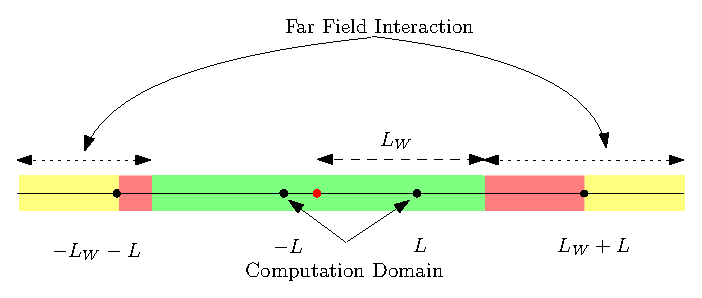
\includegraphics[width=0.8\textwidth,keepaspectratio]{figures/fig31}
\caption{To compute $I(x_i)$, we need to compute the near field interaction and local interaction using values of $u(x)$ from the green area. The values of $u(x)$ are provided in the green and red area for computing $I(x)$, $x\in [-L, L]$.}
\label{fig:fig31}
\end{figure}


Although we have used a different formula for the evaluation of the integral, we should soon realize that in the far-away off-diagonal parts, the entries are still $\nu_j h$~(except on the boundary), which the $\mathcal{H}$ matrix construction routine can still work. 


\lib{Numerical Examples}

\subsection{}

Finally, we consider the case where $\nu(y)$ grows to infinity and has heavy tail. For simplicity, we will consider the specific case where $n(\bx) = \frac{C_{d, s}}{|\bx|^{d+2s}}$, i.e., the fractional Laplacian. Fortunately we can compute  the analytical nonlocal derivative or gradient for some functions. 

For the first example, we consider $u(x)=\exp(-x^2)$ in 1D. Then we have
\begin{equation}\label{equ:u0}
	(-\Delta)^s u(0) = 2^{2s}\Gamma\left( \frac{1+2s}{2} \right)/\sqrt{\pi}
\end{equation}

For this example, since $u(x)$ decay to zero exponentially, we can assume that the far-field interaction $f^{L_W}_x=0$ is zero for sufficiently large $L_W$. The numerical value is computed using \cref{equ:I1approx,equ:I2approx,equ:I3approx} and compared with the exact value \cref{equ:u0}. The parameters are: $L_W=5.0$, $r=0.2$. The convergence plot is shown in \cref{fig:fig5}. We can see that the error converges like or better than $\mathcal{O}(h^2)$. 

\begin{figure}[H] % \usepackage{float}
\centering
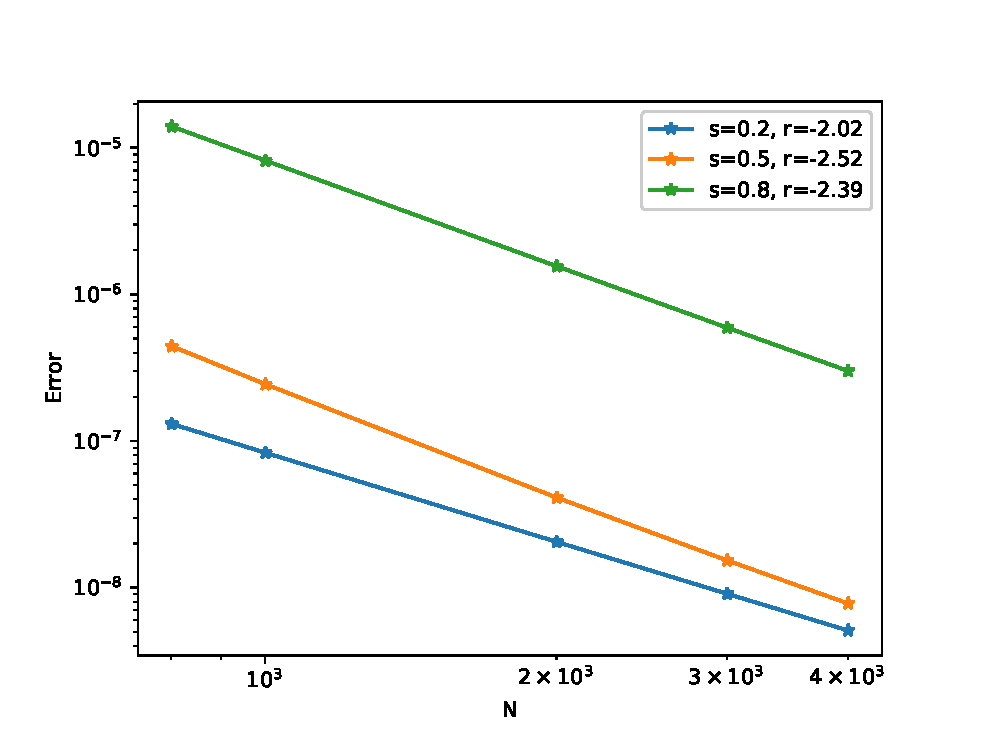
\includegraphics[width=0.8\textwidth,keepaspectratio]{figures/fig5}
\caption{Numerical error for approximating \cref{equ:u0}. The error converges like or better than $\mathcal{O}(h^2)$.}
\label{fig:fig5}
\end{figure}

We also test the scheme on a challenging problem: the fractional Poisson problem. The PDE
\begin{equation}
	\begin{cases}
		(-\Delta)^s u(x) = 1 & x\in [-1,1]\\
		u(x) = 0 & x\not\in [-1,1]
	\end{cases}
\end{equation}
has a unique solution
\begin{equation}
	u(x) = \frac{2^{2s}\Gamma(1+s)\Gamma\left( \frac{1+2s}{2} \right) }{\Gamma(1/2)} (1-x^2)^s
\end{equation}
Note that $u(x)$ is not smooth across the boundary. In fact, it only belongs to $C^{0,s}([-1,1])$, the $s$-order H\"older space. Numerical algorithms usually exhibit reduced convergence.  We use $L=1.0$ and $Lw=2.0$ so that the support of $u(x)$ is included in the near-field or local interaction. Thus we have $f_x^{L_W}=0$. Since the current implementation only supports forward computation of the nonlocal operator, i.e., given function values, the nonlocal derivative or gradient is computed, we resort to a conjugate gradient approach for recovering $u(x)$ in $[-L,L]$. 

\Cref{fig:fig6} presents the finite difference result obtained from our discretization. We can see that the convergence order is $1.0$ or less, much worse than the Poisson problem where $\mathcal{O}(h^2)$ convergence rate is typical. We need to emphasize this is a universal problem faced by many fractional Laplacian models if a simple truncation trick is used. 

\begin{figure}[H] % \usepackage{float}
\centering
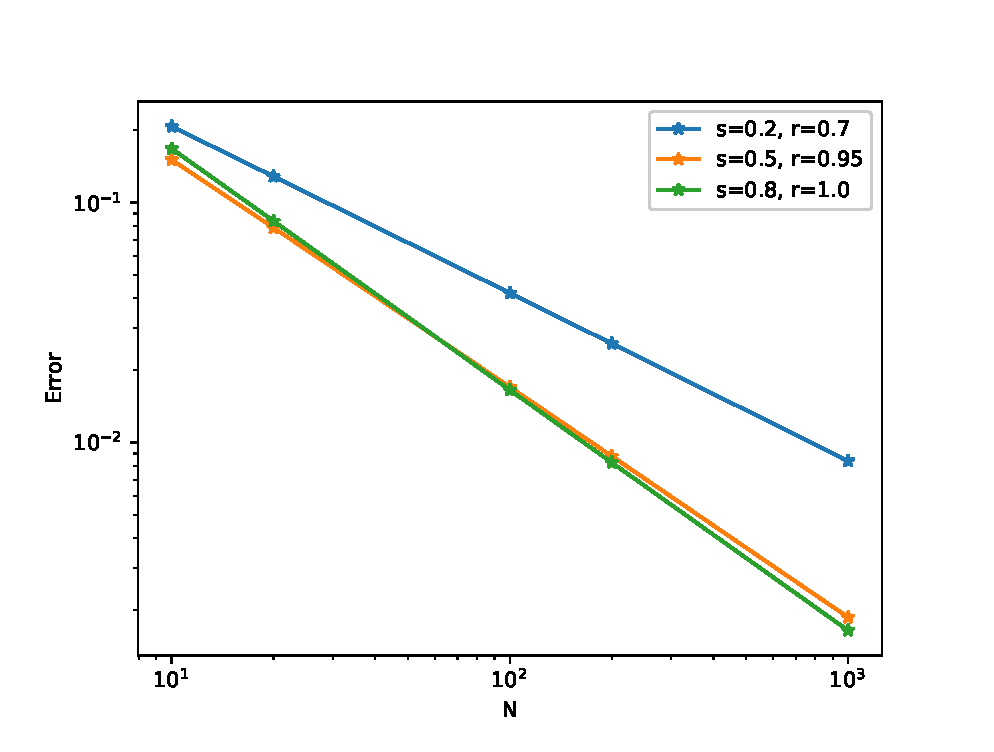
\includegraphics[width=0.45\textwidth,keepaspectratio]{figures/fig6}
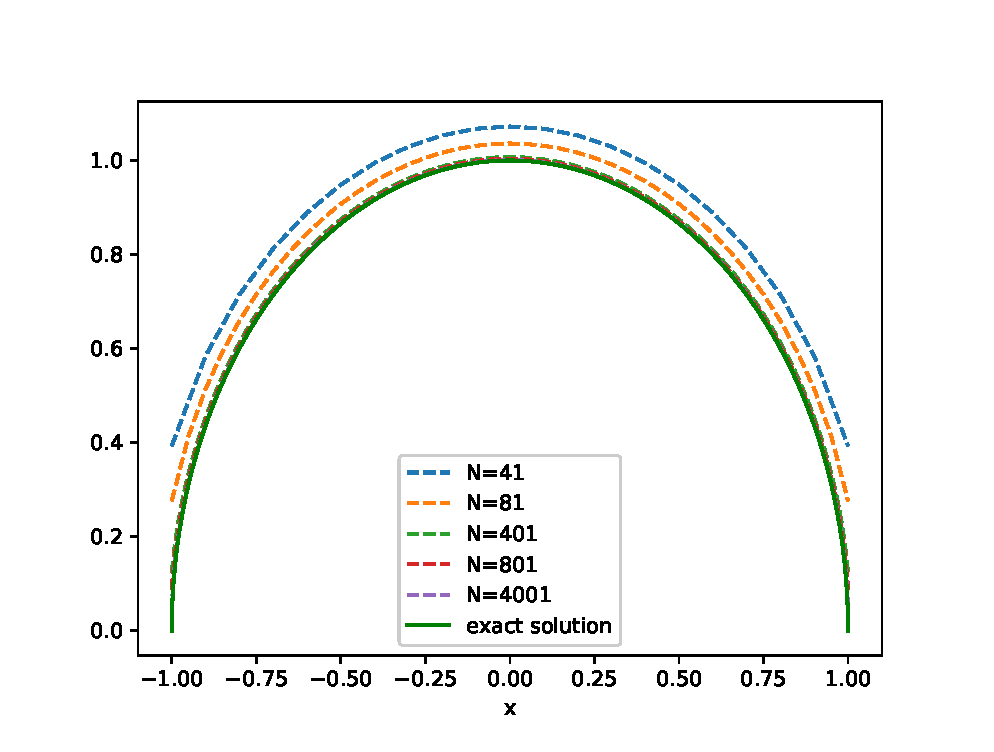
\includegraphics[width=0.45\textwidth,keepaspectratio]{figures/fig7}
\caption{The finite difference result obtained from our discretization. The convergence order is $1.0$ or less, much worse than the Poisson problem where $\mathcal{O}(h^2)$ convergence rate is typical}
\label{fig:fig6}
\end{figure}

Finally, we also consider the computation of $(-\Delta)^ u(\bx)$ in 2D, where
\begin{equation}
	u(\bx) = \frac{1}{2^{2s}\Gamma(1+s)^2} ((1-|\bx|^2)^s_+
\end{equation}

The analytically result is known for $|\bx|\leq 1$, which is
\begin{equation}\label{equ:u1}
	(-\Delta)^s u(\bx) = 1\quad |\bx|\leq 1
\end{equation}
The numerical result is shown in \cref{fig:fig8}. Near the boundary, due to the nonsmoothness of $u(\bx)$, the algorithm is having a hard time computing the nonlocal gradient and therefore we see the oscillatory behavior. However, the computation for the region near the center is  good, which does not suffer much from the far-away contribution from nonsmooth boundaries. In the center the error is only $4\%$. We used $L_W=2.0$ and $L=1.0$ in this case.  

\begin{figure}[H] % \usepackage{float}
\centering
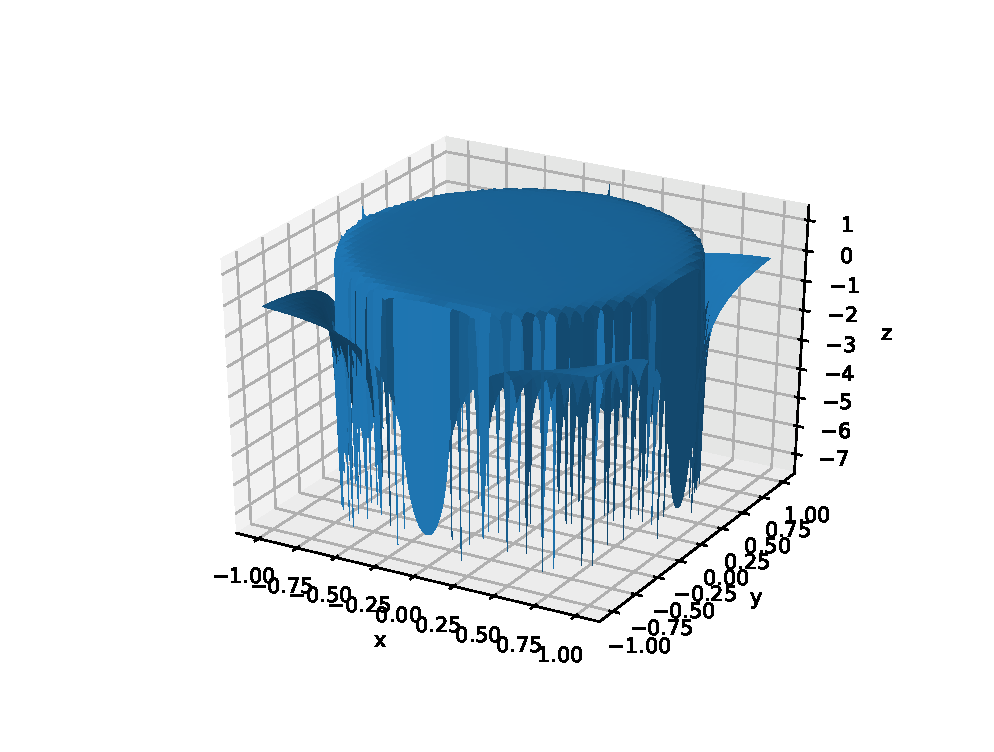
\includegraphics[width=0.8\textwidth,keepaspectratio]{figures/fig8}
\caption{Numerical evaluation of \cref{equ:u1}. Near the boundary, due to the nonsmoothness of $u(\bx)$, the algorithm is having a hard time computing the nonlocal gradient and therefore we see the oscillatory behavior. However, the computation for the region near the center is  good, which does not suffer much from the far-away contribution from nonsmooth boundaries. In the center the error is only $4\%$.}
\label{fig:fig8}
\end{figure}

These numerical examples demonstrates that the numerical scheme also works for $\nu(y)$ which has heavy tails. 

\end{document}